\documentclass[aspectratio=169,12pt]{beamer}
\usetheme{Madrid}
\usecolortheme{default}
\setbeamertemplate{navigation symbols}{}
\setbeamertemplate{footline}[frame number]

\usepackage{graphicx}
\usepackage{booktabs}
\usepackage{amsmath}
\usepackage{xcolor}

\definecolor{myblue}{RGB}{51,102,187}
\definecolor{mygreen}{RGB}{46,139,87}
\definecolor{myred}{RGB}{204,51,51}

\title{Fault-Tolerant Multi-GPU LLM Serving\\with Adaptive KV-Cache Checkpointing}
\subtitle{Progress Update}
\author{Yi Zhong}
\date{\today}

\begin{document}

% ============================================================
\begin{frame}
\titlepage
\end{frame}

% ============================================================
\begin{frame}{Problem}
\begin{itemize}
    \item Single-node multi-GPU LLM serving: replicas can fail (GPU reset, OOM, driver crash...)
    \item Failure $\Rightarrow$ lost capacity $\Rightarrow$ interrupted streams, SLO violations, goodput drop
    \item Naive checkpoint: too frequent = overhead; too rare = long recovery
\end{itemize}

\vspace{0.5em}
\textbf{Core question:} How to jointly optimize \textcolor{myblue}{routing}, \textcolor{myblue}{admission}, and \textcolor{myblue}{adaptive checkpointing} to maximize goodput while meeting SLOs under failures?
\end{frame}

% ============================================================
\begin{frame}{Our System}
\begin{columns}[T]
\begin{column}{0.55\textwidth}
\textbf{Two components:}
\begin{enumerate}
    \item \textbf{Benders-based robust scheduler}
    \begin{itemize}
        \item Periodic decision epochs
        \item Master: admission + routing
        \item Subproblem: verify recovery feasibility for each failure scenario
        \item Pooled-flow recovery screening
    \end{itemize}
    \item \textbf{Adaptive checkpoint policy}
    \begin{itemize}
        \item Runtime-local, per-request
        \item Publish KV blocks when: \\
              $\Delta\text{replay\_saved} > \Delta\text{load} + \lambda \cdot \Delta\text{ckpt\_overhead}$
        \item Early: skip (cheap to replay)
        \item Late: checkpoint (expensive to lose)
    \end{itemize}
\end{enumerate}
\end{column}
\begin{column}{0.4\textwidth}
\textbf{Baselines:}
\begin{itemize}
    \item \textbf{No-FT}: no fault tolerance
    \item \textbf{Fixed-Low-CKPT}: low-freq fixed ckpt
    \item \textbf{Fixed-High-CKPT}: high-freq fixed ckpt (every block)
    \item \textbf{Robust-Routing-Only}: Benders routing + fixed low ckpt
    \item \textbf{Checkpoint-Only}: adaptive ckpt + greedy routing
\end{itemize}
\end{column}
\end{columns}
\end{frame}

% ============================================================
\begin{frame}{Experiment Setup}
\begin{columns}[T]
\begin{column}{0.5\textwidth}
\textbf{Hardware \& Model}
\begin{itemize}
    \item Llama-3.2-1B-Instruct
    \item 2 GPUs (data-parallel replicas)
    \item 8GB checkpoint pool (host RAM)
\end{itemize}

\vspace{0.5em}
\textbf{Workloads}
\begin{itemize}
    \item W1: Short Interactive (P:50--200, G:20--100)
    \item W2: Long Generation (P:200--500, G:200--500)
    \item W3: Bursty Mixed (P:50--500, G:20--500)
\end{itemize}
\end{column}
\begin{column}{0.45\textwidth}
\textbf{Load levels}: Low (1 rps), Medium (3), High (5)

\vspace{0.5em}
\textbf{Fault injection}
\begin{itemize}
    \item none, F1\_Early (15s), F2\_Mid (30s), F3\_Late (50s)
    \item Kill one GPU replica
\end{itemize}

\vspace{0.5em}
\textbf{SLO targets}
\begin{itemize}
    \item TTFT: 2s
    \item TPOT: 100ms
    \item Failover gap: 3s
\end{itemize}

\vspace{0.5em}
\textbf{Duration}: 70s per run
\end{column}
\end{columns}
\end{frame}

% ============================================================
\begin{frame}{Experiments Overview}
\centering
\begin{tabular}{lll}
\toprule
\textbf{Experiment} & \textbf{Goal} & \textbf{Key Metric} \\
\midrule
E1: Main & End-to-end comparison & Goodput, SLO violation, failover gap \\
E2: Recovery & Where does recovery time go? & Time breakdown \\
E3: Ablation & Routing vs Checkpoint contribution & Goodput (component-wise) \\
E4: Tradeoff & Checkpoint overhead vs recovery benefit & Goodput + gap \\
E5: Controller & Is the solver fast enough? & Solver latency \\
\bottomrule
\end{tabular}
\end{frame}

% ============================================================
\begin{frame}{E1: Goodput --- No Fault}
\centering
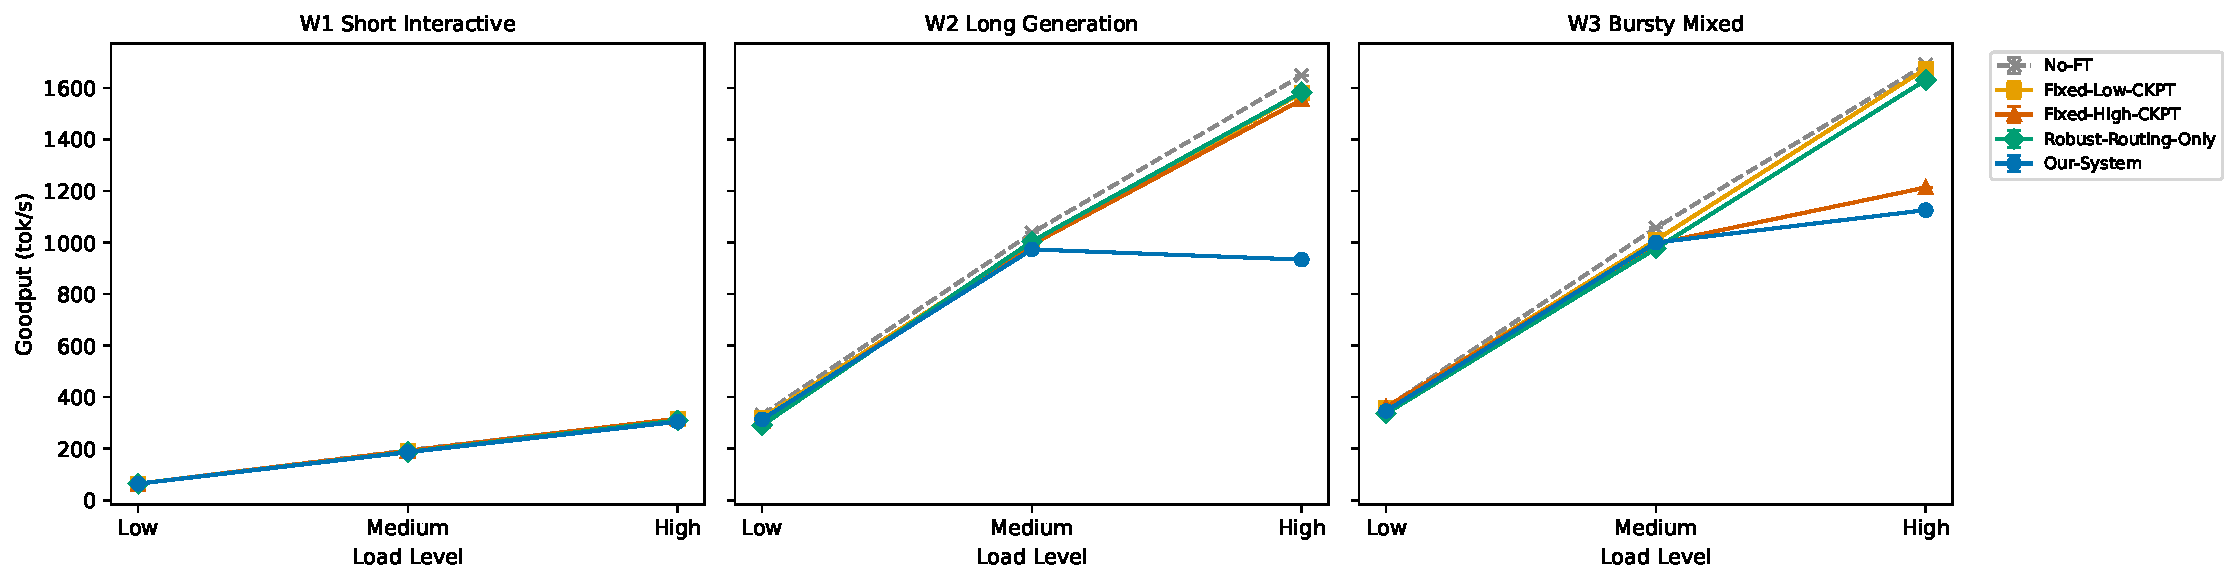
\includegraphics[width=0.95\textwidth]{../figures/E1_Main/goodput_by_load_none.pdf}

\vspace{0.3em}
\begin{itemize}
    \item All methods $\approx$ No-FT in normal case $\Rightarrow$ \textcolor{mygreen}{our system has negligible overhead}
    \item Exception: \textcolor{myred}{Fixed-High-CKPT} drops $\sim$40\% on W2/High (960 vs 1640 tok/s) due to copy overhead
\end{itemize}
\end{frame}

% ============================================================
\begin{frame}{E1: Goodput --- With Fault (F2\_Mid)}
\centering
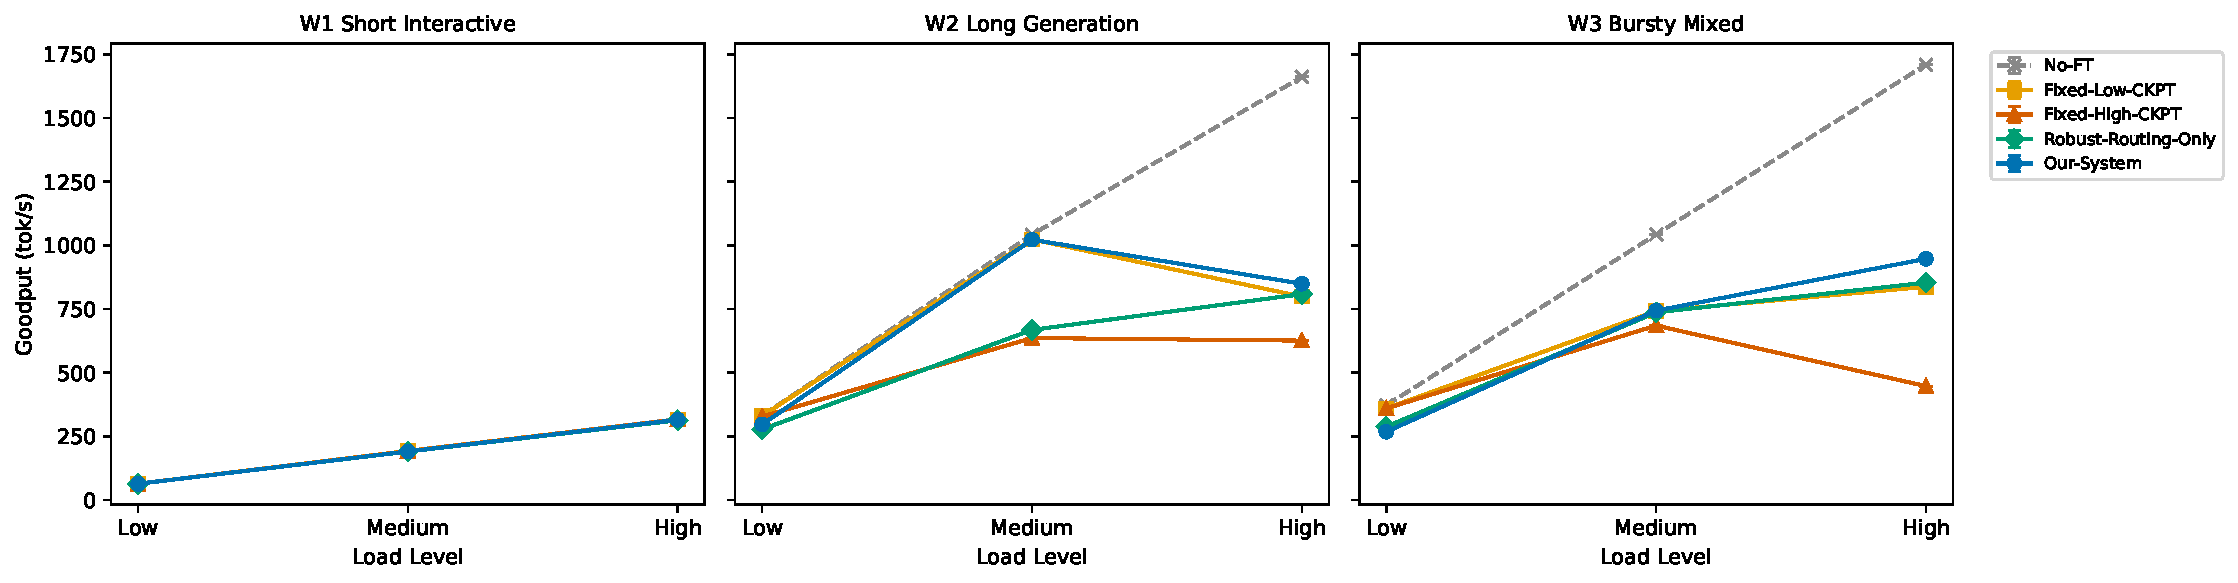
\includegraphics[width=0.95\textwidth]{../figures/E1_Main/goodput_by_load_F2_Mid.pdf}

\vspace{0.3em}
\begin{itemize}
    \item No-FT goodput looks high but it \textcolor{myred}{drops requests silently} (completion rate $\sim$98\%, 0\% failover)
    \item Our-System $\approx$ Fixed-Low on W2/Med ($\sim$1040), but 100\% completion rate
    \item Fixed-High-CKPT worst: overhead + slow recovery
\end{itemize}
\end{frame}

% ============================================================
\begin{frame}{E1: SLO Violations}
\begin{columns}[c]
\begin{column}{0.48\textwidth}
\centering
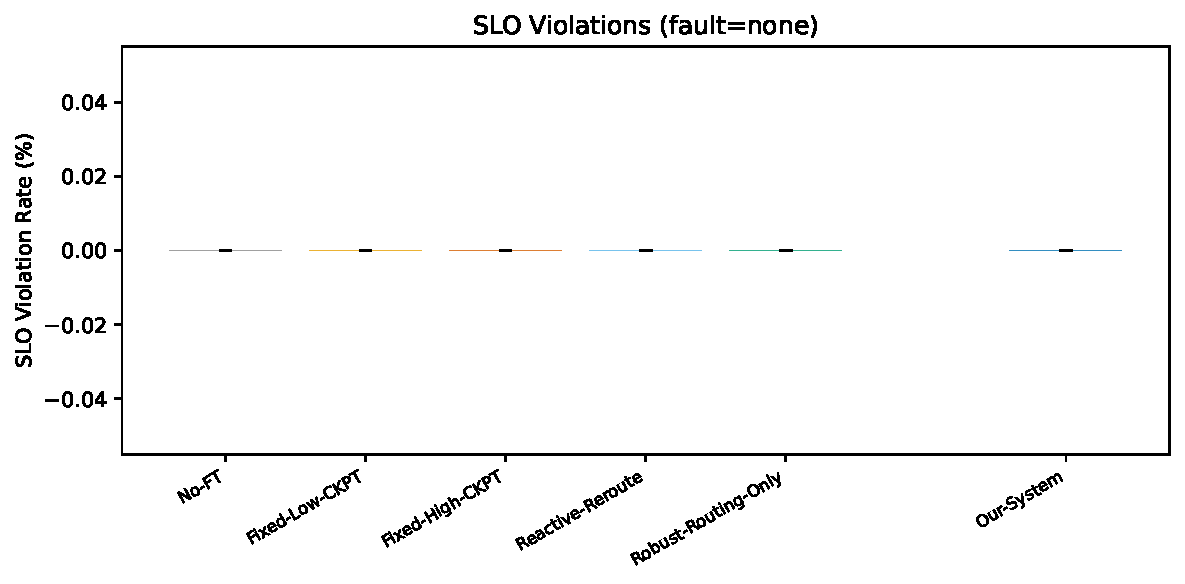
\includegraphics[width=\textwidth]{../figures/E1_Main/slo_violation_none.pdf}
\end{column}
\begin{column}{0.48\textwidth}
\centering
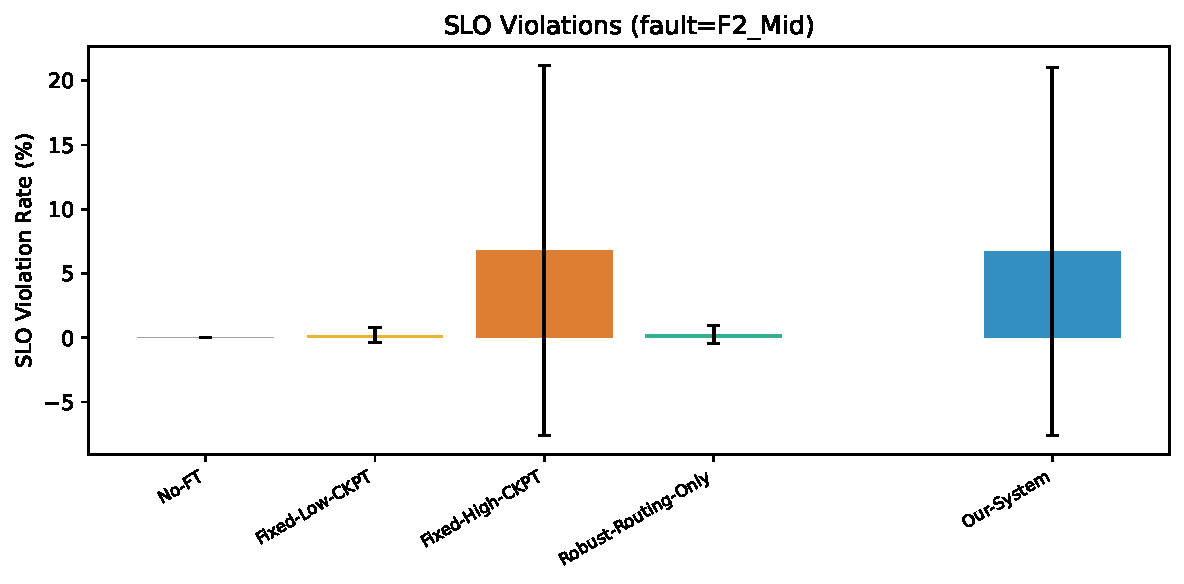
\includegraphics[width=\textwidth]{../figures/E1_Main/slo_violation_F2_Mid.pdf}
\end{column}
\end{columns}

\vspace{0.3em}
\begin{itemize}
    \item No fault: all methods 0\% violation
    \item With fault: \textcolor{myred}{Fixed-High-CKPT} up to $\sim$7\% (worst case 20\%+); \textcolor{mygreen}{Our-System $\approx$ 0\%}
\end{itemize}
\end{frame}

% ============================================================
\begin{frame}{E1: Failover Gap (p95)}
\centering
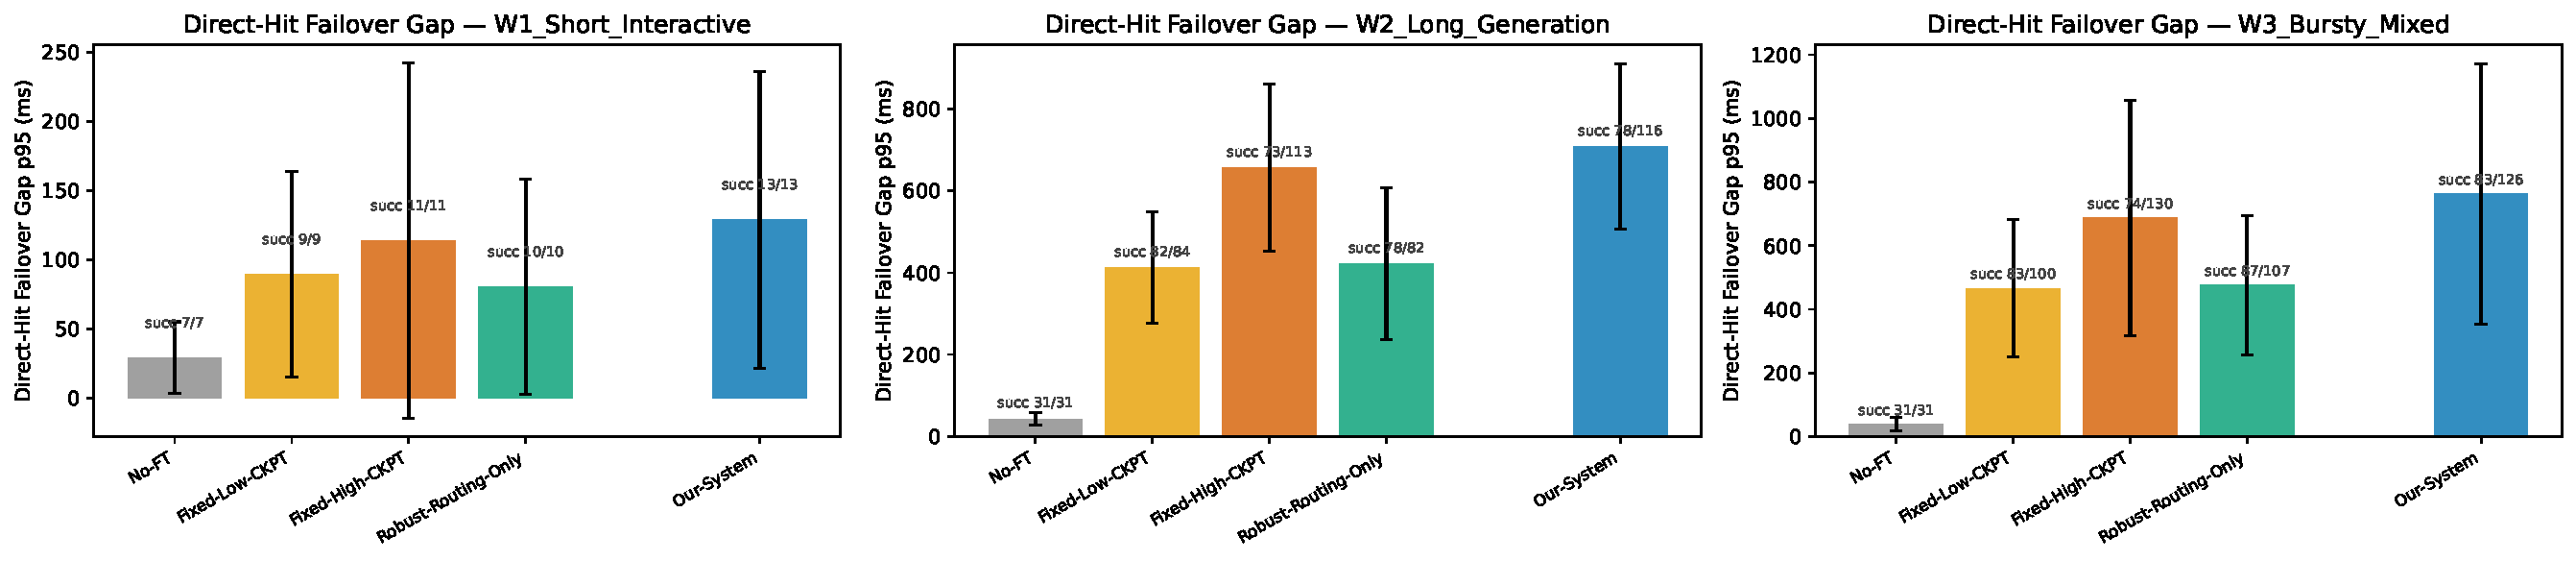
\includegraphics[width=0.95\textwidth]{../figures/E1_Main/failover_gap_p95.pdf}

\vspace{0.3em}
\begin{itemize}
    \item No-FT: 0\% recovery on W2/W3 (succ 0/34, 0/27)
    \item Fixed-High-CKPT: highest gap ($\sim$700ms W2) + lowest success rate (77/117 = 66\%)
    \item \textcolor{mygreen}{Our-System}: moderate gap + \textbf{highest success rate} (W3: 90/97 = 93\%)
\end{itemize}
\end{frame}

% ============================================================
\begin{frame}{E2: Recovery Time Breakdown}
\centering
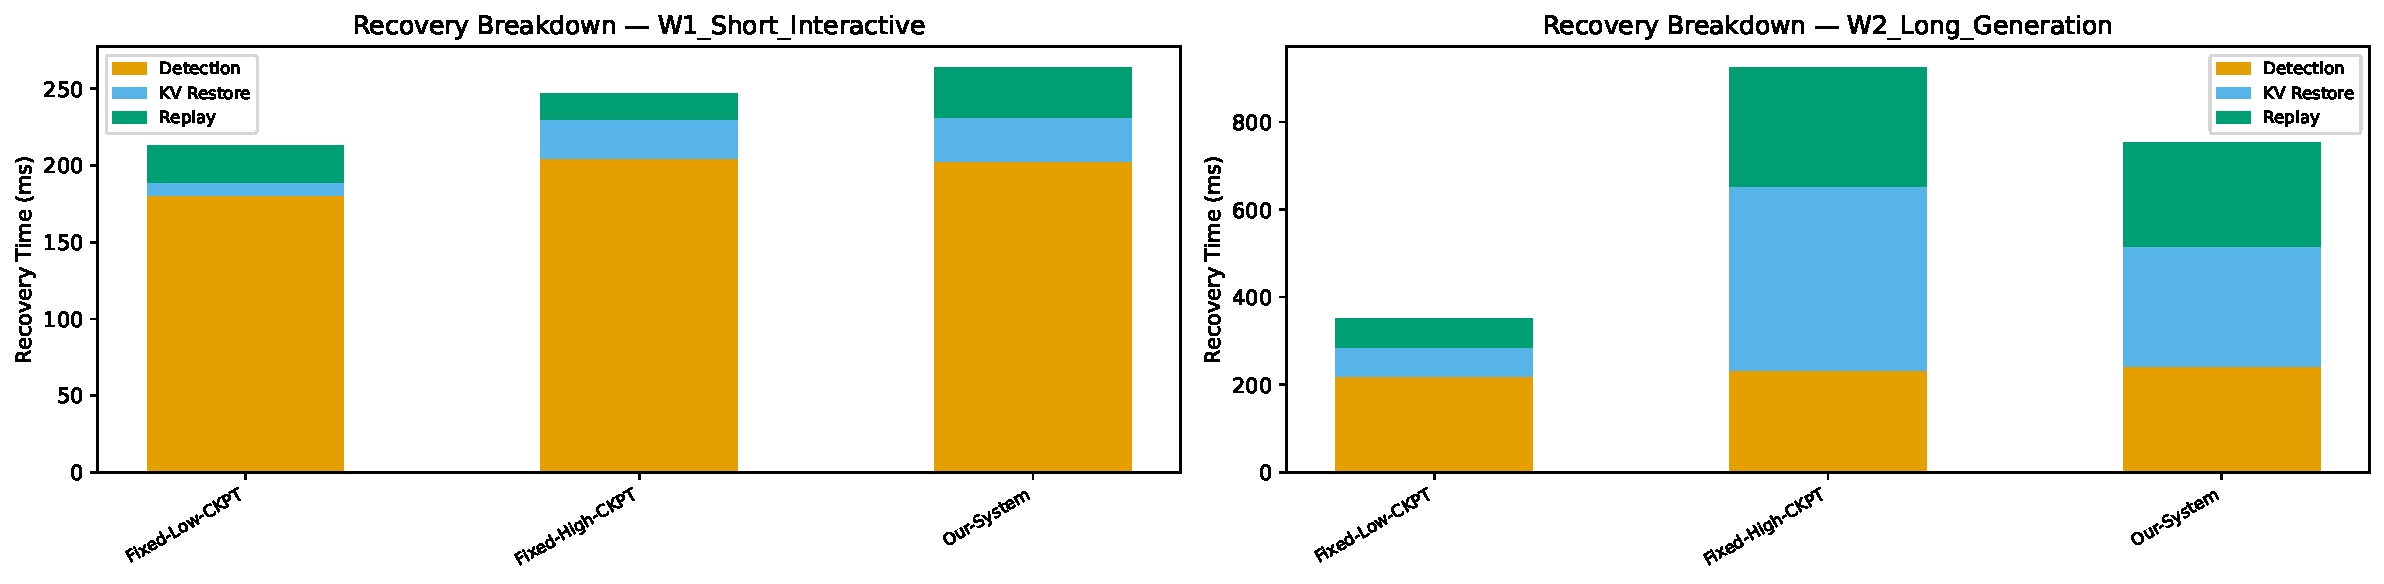
\includegraphics[width=0.85\textwidth]{../figures/E2_Recovery/recovery_breakdown.pdf}

\vspace{0.3em}
\begin{itemize}
    \item W1 (short): detection dominates ($\sim$200ms), all methods similar
    \item W2 (long): \textcolor{myred}{Fixed-High-CKPT $\sim$830ms} (KV restore too large); Our-System $\sim$330ms
    \item Adaptive checkpoint: not too much to load, not too much to replay $\Rightarrow$ \textcolor{mygreen}{sweet spot}
\end{itemize}
\end{frame}

% ============================================================
\begin{frame}{E3: Ablation --- With Fault (F2\_Mid)}
\centering
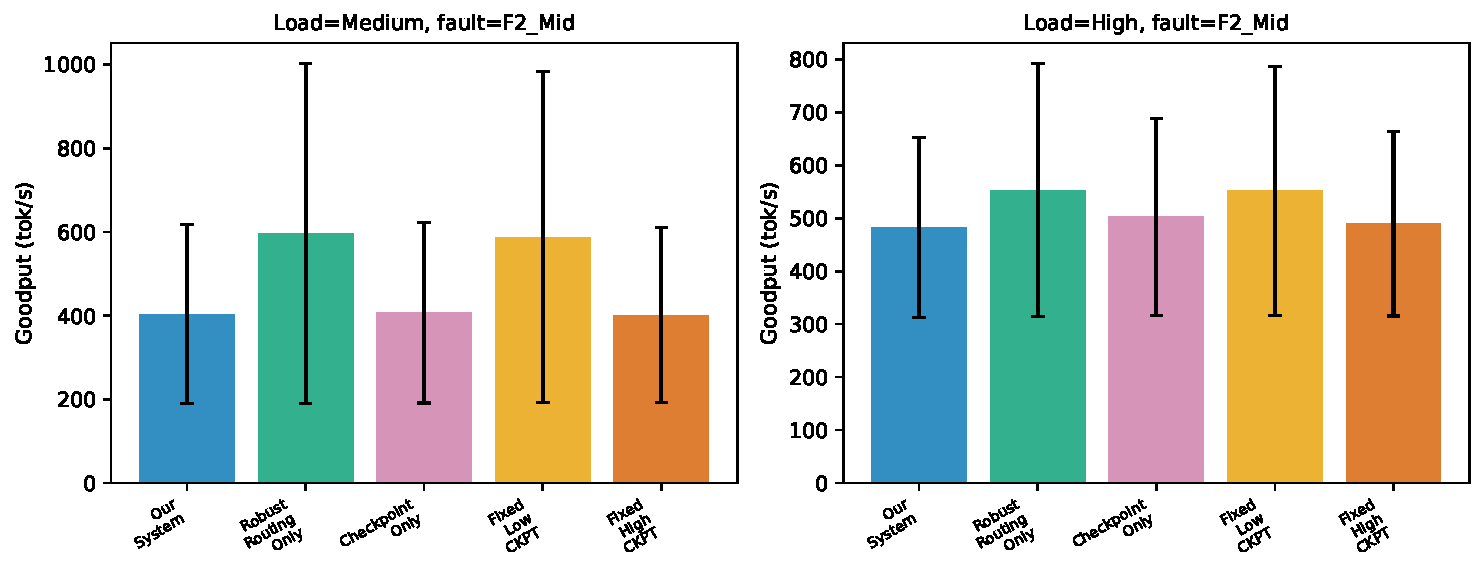
\includegraphics[width=0.85\textwidth]{../figures/E3_Ablation/ablation_F2_Mid.pdf}

\vspace{0.3em}
\begin{itemize}
    \item W1 (short tasks): all methods similar --- short tasks are easy to recover
    \item W2/Med: Our-System $\approx$ Checkpoint-Only ($\sim$1040) $\gg$ Robust-Routing-Only ($\sim$666)
    \item \textbf{Adaptive checkpoint is the primary contributor}; routing helps more at high load
\end{itemize}
\end{frame}

% ============================================================
\begin{frame}{E3: Ablation --- No Fault}
\centering
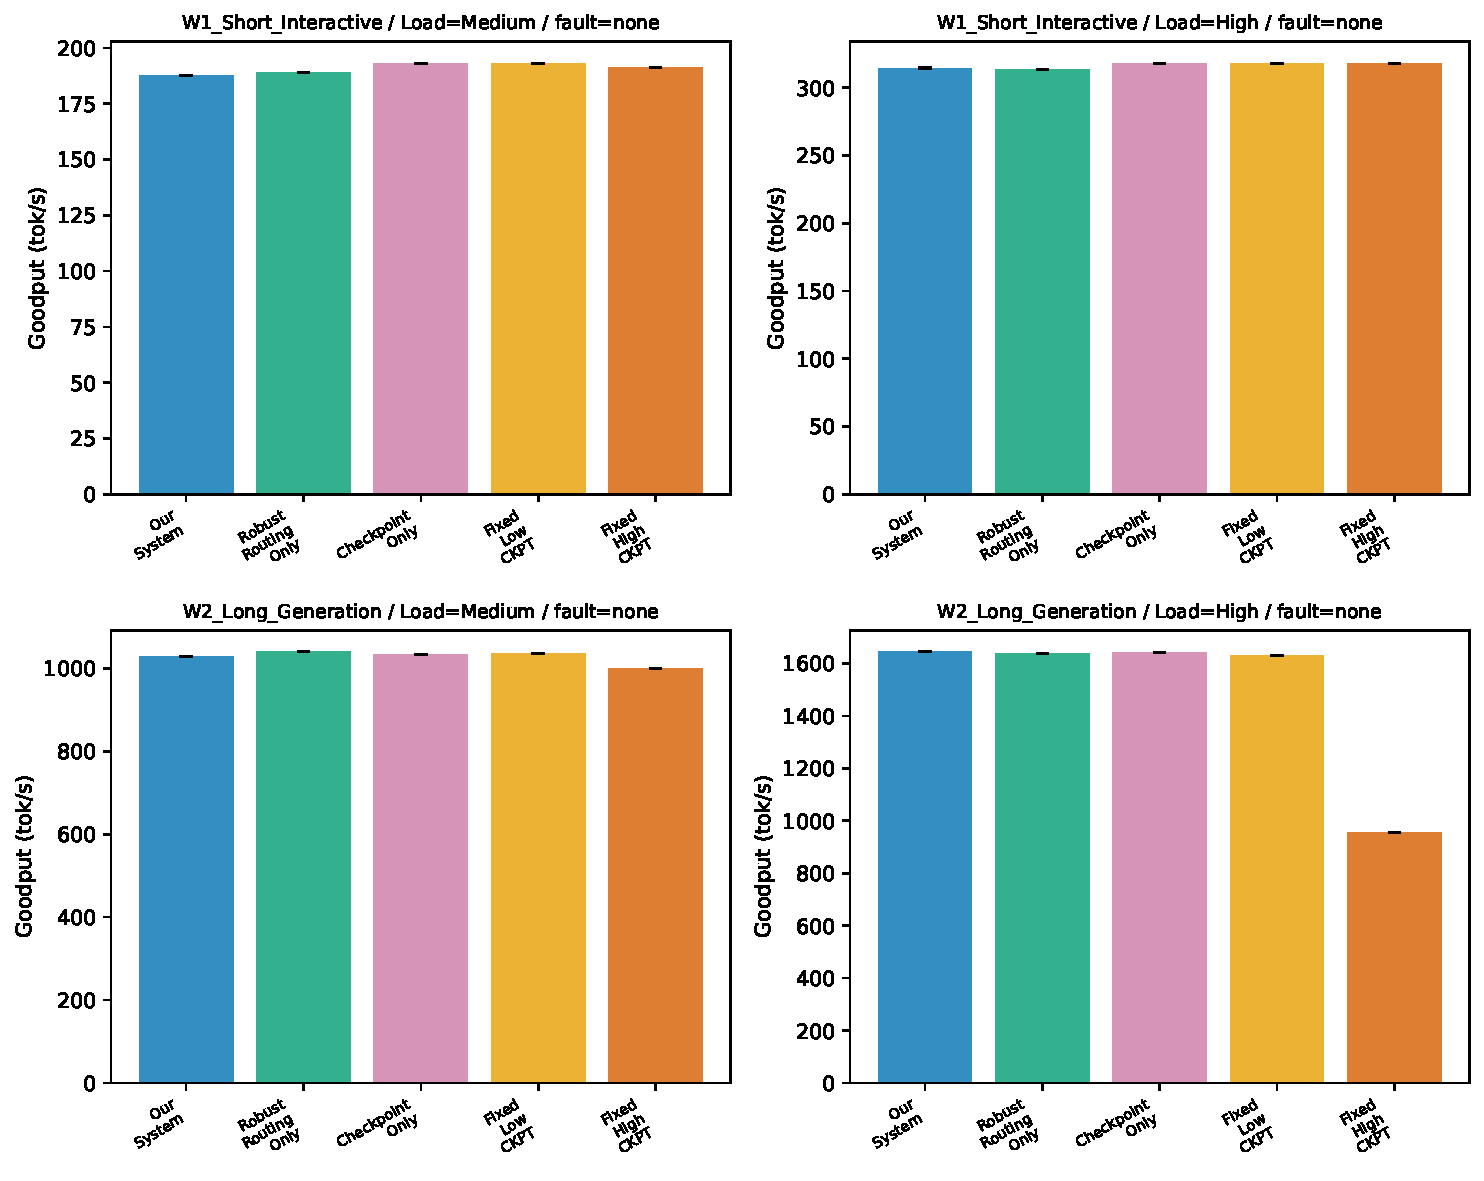
\includegraphics[width=0.85\textwidth]{../figures/E3_Ablation/ablation_none.pdf}

\vspace{0.3em}
\begin{itemize}
    \item Normal case: Our-System / Robust-Routing / Checkpoint-Only / Fixed-Low all comparable
    \item \textcolor{myred}{Fixed-High-CKPT}: W2/High only $\sim$960 vs others $\sim$1640 ($-$40\% from copy overhead alone)
\end{itemize}
\end{frame}

% ============================================================
\begin{frame}{E4: Checkpoint Overhead vs Recovery Benefit}
\centering
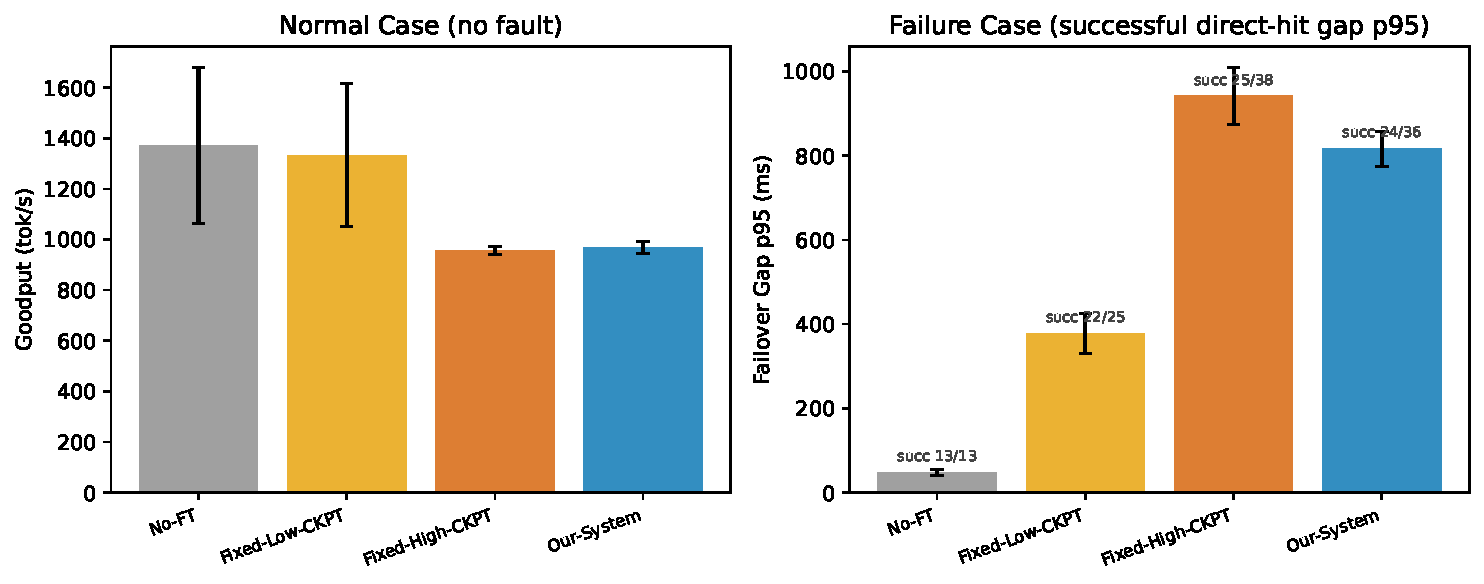
\includegraphics[width=0.85\textwidth]{../figures/E4_Checkpoint_Tradeoff/checkpoint_tradeoff.pdf}

\vspace{0.3em}
\begin{itemize}
    \item \textbf{Left (normal)}: Fixed-High-CKPT loses $\sim$30\% goodput; others $\approx$ No-FT
    \item \textbf{Right (fault)}: No-FT: 0/10 recovery; Fixed-High: 22/39 (56\%), gap $\sim$800ms
    \item \textcolor{mygreen}{Our-System: 27/27 (100\%) recovery, gap $\sim$500ms} --- best on both axes
\end{itemize}
\end{frame}

% ============================================================
\begin{frame}{E5: Controller Overhead}
\centering
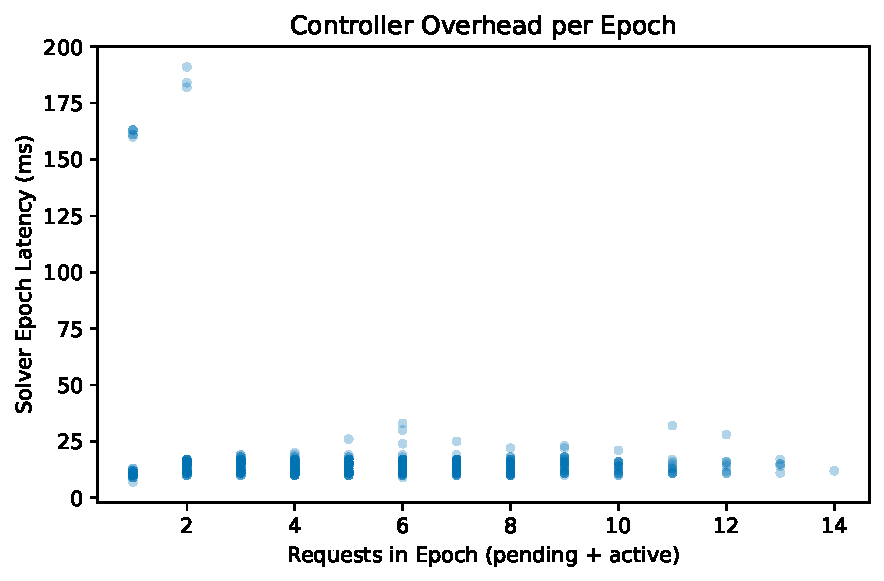
\includegraphics[width=0.65\textwidth]{../figures/E5_Controller/controller_overhead.pdf}

\vspace{0.3em}
\begin{itemize}
    \item Median solver latency: \textbf{$\sim$15ms per epoch}, regardless of request count (1--12)
    \item Outliers at 160--180ms: cold start (first 1--2 calls), can be eliminated by warmup
    \item Acceptable overhead for online serving (decode step $\sim$ms scale)
\end{itemize}
\end{frame}

% ============================================================
\begin{frame}{Summary}

\textbf{Key findings:}
\begin{enumerate}
    \item \textbf{Normal case}: Our system has near-zero overhead vs No-FT
    \item \textbf{Fault case}: Highest recovery success rate + lowest SLO violations
    \item \textbf{Checkpoint $\neq$ more is better}: Fixed-High-CKPT hurts both goodput and recovery
    \item \textbf{Adaptive checkpoint is the main contributor}; robust routing provides additional robustness at high load
    \item \textbf{Solver overhead is small}: $\sim$15ms per epoch
\end{enumerate}

\vspace{0.5em}
\textbf{Next steps:}
\begin{itemize}
    \item Scale to more GPUs (4--8) to show routing benefits
    \item More seeds for statistical significance
    \item Stronger cut generation (beyond no-good cuts)
\end{itemize}
\end{frame}

\end{document}